\section{ODD for StationSim GCS}\label{sec:stationsim}

\subsection{Overview}\label{sub:stationsim:overview}

\subsubsection{Purpose and patterns}\label{subs:stationsim:overview:purpose}

StationSim GCS is an updated version of the StationSim model.
The original StationSim aimed to simulate the motion of pedestrians across a
hypothetical rectangular station with 3 entrances on one side and 2 exits on the
opposite side as shown in Figure~\ref{fig:stationsim_env}.
The new StationSim GCS also aims to simulation the motion of pedestrians across
a station; however, in this case the model is based on the real-world example of
Grand Central Station in New York, focusing specifically on the concourse area
highlighted in Figure~\ref{fig:gcs_concourse}.
This is reflected in the simulation environment shown in
Figure~\ref{fig:stationsim_gcs_env}.
The environment consists of X gates which act simultaneously as both entrances
and exits.
Each pedestrian in the simulation is assigned an entrance and an exit and, upon
entering the environment, seeks to move as directly as possible towards their
assigned exit without colliding with other pedestrians.
Where collisions are more likely to occur (e.g. close to entrances/exits and
around solid obstacles), we typically observe crowding as population densities
increase.

\todo{The new version of ODD has introduced patters (from pattern-oriented
modelling) --- what are the patterns?}

\begin{figure}[h]
    \centering
    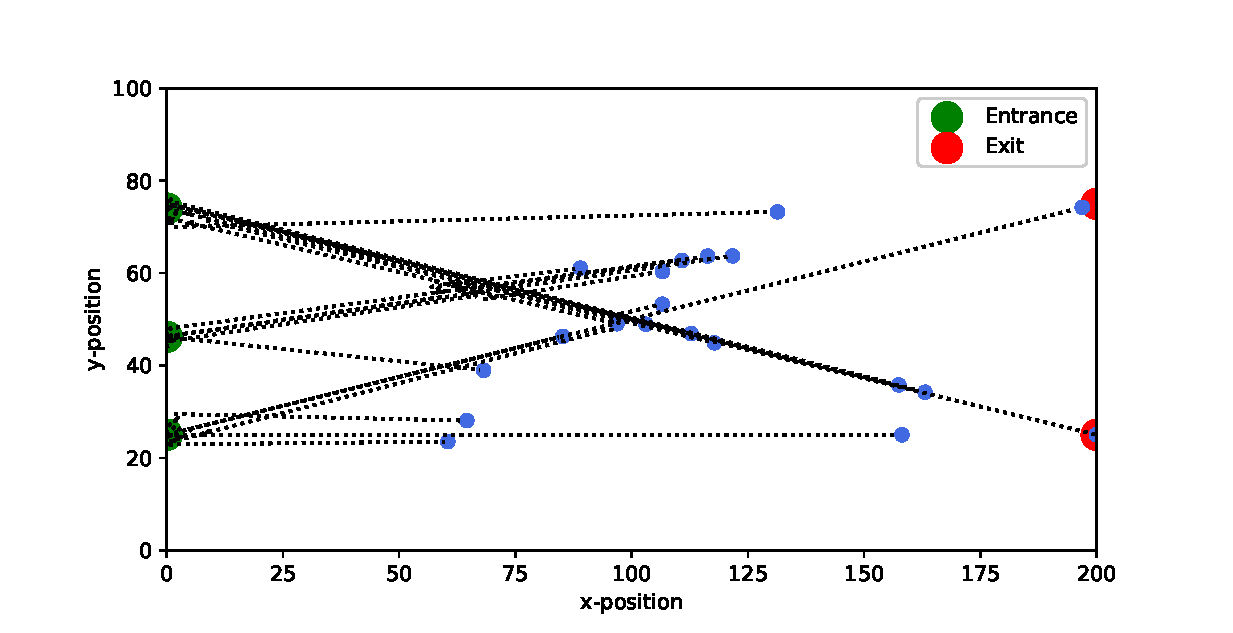
\includegraphics[width=0.7\textwidth]{sample_model_run}
    \caption{Layout of environment in original StationSim
    model.}\label{fig:stationsim_env}
\end{figure}

\begin{figure}[h]
    \centering
    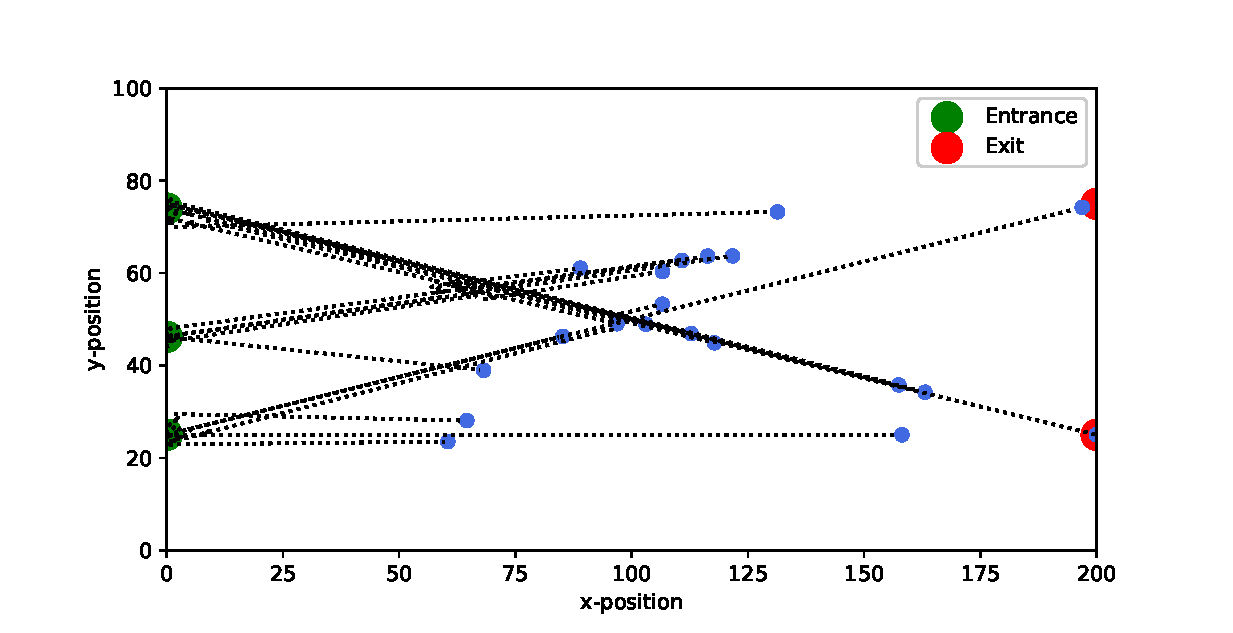
\includegraphics[width=0.7\textwidth]{sample_model_run}
    \caption{Layout of Grand Central Station
    concourse.}\label{fig:gcs_concourse}
\end{figure}

\begin{figure}[h]
    \centering
    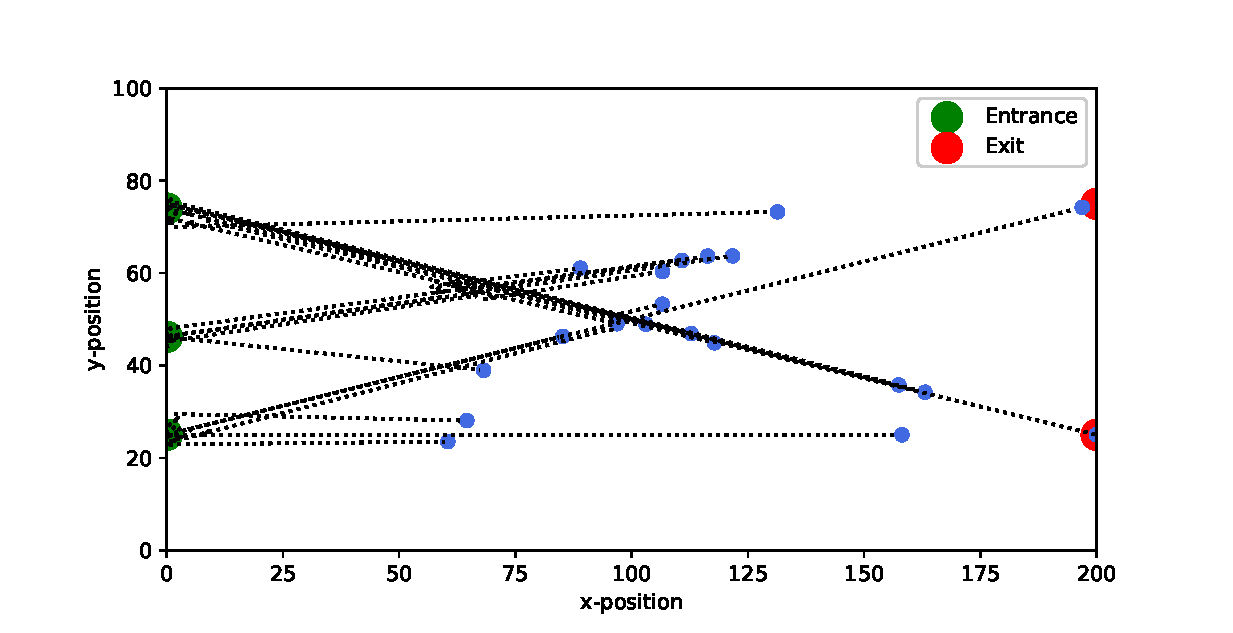
\includegraphics[width=0.7\textwidth]{sample_model_run}
    \caption{Layout of environment in StationSim GCS
    model.}\label{fig:stationsim_gcs_env}
\end{figure}

\subsubsection{Entities, state variables and
scales}\label{subs:stationsim:overview:entities}

The StationSim GCS model is made up of 4 different types of entities:
\begin{enumerate}
    \item Agents,
    \item The environment,
    \item Gates around the edge of the environment, and
    \item Obstacles in the environment.
\end{enumerate}
These entities aim to simulate the scenario outlined in
Section~\ref{sub:stationsim:overview}.
The agents in this model represent pedestrians; these are portrayed as
two-dimensional circular entities with finite radius.
The variables pertaining to these agents can be found in
Table~\ref{tab:agent_variables}.
The environment in this model represents the concourse of Grand Central Station
in New York; this is portrayed as two-dimensional continuous space bounded by
rectangular walls within which agents may move.
The model is designed such that the left-hand side of the environment
represents the South side of the concourse, the right-hand side the North side,
the top side the West side and the bottom side the East side.
The variables pertaining to the environment entity can be found in
Table~\ref{tab:environment_variables}.

\begin{table}
    \centering
    \begin{tabularx}{\textwidth}{lX}
        \toprule
        Variable Name & Description \\
        \midrule
        \texttt{location} & Agent's $x$-$y$ coordinates in 2-dimensional
                            continuous space; bounded by the height and width of
                            the environment \\
        \texttt{status} & Agent's status; 0 indicates agent has not started, 1
                          indicates agent is active, 2 indicates agent has
                          finished \\
        \texttt{size} & Radius of agent's circular body \\
        \texttt{speed} & Agent's speed; indicative of the distance covered by an
                         agent in a single time-step \\
        \texttt{unique\_id} & Unique numerical identifier for a specific agent
                              in a model \\
        \texttt{gate\_in} & Number of the gate through which of the gates the
                            agent enters the environment ($0 \leq n \leq 9$) \\
        \texttt{gate\_out} & Number of the gate through which of the gates the
                             agent exits the environment ($0 \leq n \leq 9$) \\
        \texttt{loc\_desire} & $x$-$y$ coordinate of the agent's target
                               destination; defined by taking the $x$-$y$
                               coordinates of \texttt{gate\_out} and adding some
                               uniformly distributed random noise \\
        \bottomrule
    \end{tabularx}
    \caption{Table of state variables pertaining to gate
    entities.}\label{tab:agent_variables}
\end{table}

\begin{table}
    \centering
    \begin{tabularx}{\textwidth}{lX}
        \toprule
        Variable Name & Description \\
        \midrule
        \texttt{height} & Environment's height \\
        \texttt{width} & Environment's width \\
        \texttt{gates\_in} & Number of gates through which agents can enter the
                             environment \\
        \texttt{gates\_out} & Number of gates through which agents can exit the
                              environment \\
        \bottomrule
    \end{tabularx}
    \caption{Table of state variables pertaining to the environment
    entity.}\label{tab:environment_variables}
\end{table}

Along the edge of these boundaries are located gates: one gate is located on the
South side, five gates are located on the North side, two gates are located on
the West side and two gates are located on the East side.
The gates are points along the boundary of the environment at which agents may
either enter or exit.
These have specific fixed $x$-$y$ coordinates.
Upon initialisation, each agent is provided with a start gate and end gate, from
which it draws its initial location and target destination; in defining its
target destination, the agent introduces some random noise to the $x$-$y$
coordinate in order to emulate the non-zero width of the gate.
The variables pertaining to the gate entities can be found in
Table~\ref{tab:gate_variables}.

\begin{table}
    \centering
    \begin{tabularx}{\textwidth}{lX}
        \toprule
        Variable Name & Description \\
        \midrule
        \texttt{location} & Gate's $x$-$y$ coordinates; restricted to one of ten
                            distinct locations on the boundary of the
                            environment \\
        \bottomrule
    \end{tabularx}
    \caption{Table of state variables pertaining to gate
    entities.}\label{tab:gate_variables}
\end{table}

The environment also contains a single obstacle which represents a clock.
As shown in Figure~\ref{fig:gcs_concourse}, this lies in the centre of the
concourse.
From a model architecture perspective, this obstacle is treated as a stationary
agent; other agents therefore treat it as they would any other agent and make
efforts to avoid colliding with it.
The variables pertaining to the obstacle entity can be found in
Table~\ref{tab:obstacle_variables}.

\begin{table}
    \centering
    \begin{tabularx}{\textwidth}{lX}
        \toprule
        Variable Name & Description \\
        \midrule
        \texttt{location} & Obstacle's $x$-$y$ coordinates \\
        \texttt{size} & Radius of obstacle's circular body \\
        \texttt{speed} & Speed of agent characterising the obstacle; fixed value
                         of 0 \\
        \bottomrule
    \end{tabularx}
    \caption{Table of state variables pertaining to the obstacle
    entity.}\label{tab:obstacle_variables}
\end{table}

Of the variables detailed for each of the entities in
Tables~\ref{tab:agent_variables},~\ref{tab:environment_variables},~\ref{tab:gate_variables}
and~\ref{tab:obstacle_variables}, the majority are set
to fixed values upon model initialisation.
The variables that change as the model runs are the \texttt{location} and
\texttt{status} variables pertaining to the agent entities.

\subsubsection{Process overview and
scheduling}\label{subs:stationsim:overview:process}

\begin{figure}[h]
    \centering
    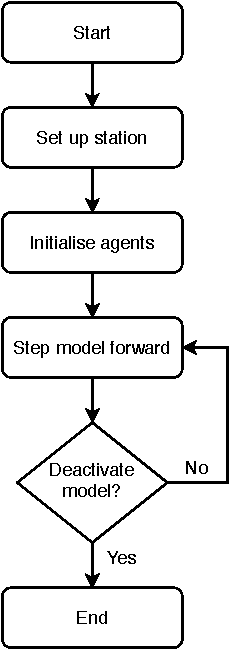
\includegraphics[width=0.5\textwidth]{stationsim_gcs-main_algorithm}
    \caption{Flow diagram of StationSim GCS}\label{fig:flow:stationsim}
\end{figure}

\subsection{Design Concepts}\label{sub:stationsim:design_concepts}

Of the design concepts outlined in~\cite{grimm2010odd}, the following are
considered relevant to this model:
\begin{enumerate}
    \item Emergence
    \item Adaptation
    \item Prediction
    \item Sensing
    \item Interaction
    \item Stochasticity
    \item Observation
\end{enumerate}

As outlined in Section~\ref{subs:stationsim:overview:process}, in each time-step
agents engage in collision avoidance (both with each other and with walls and
obstacles).
This is achieved by \emph{predicting} the paths that agents would take if they
were to continue moving towards their target destinations; this is made possible
through the use of a $k$-d tree which emulates a form of \emph{sensing} whereby
each agent is aware of the position of other agents who are likely to collide
with them.
In cases where collisions would occur, the agent paths are \emph{adapted}.
Such adaptations can be considered an indirect form of \emph{interaction}
between an agent and other agents (as well as stationary objects in the
environment).

\emph{Stochasticity} is incorporated in the model in number of different ways.
Upon initialisation, agents are randomly allocated an entrance gate and an exit
gate; entrance gates are sampled from a uniform discrete distribution, and exit
gates are sampled from a uniform discrete distribution excluding the gate
through which the agent is entering.
In cases where pedestrians are predicted to collide, part of the avoidance
process involves the addition of normally distributed random noise to the
agent's movement vector.
Finally the time at which each agent enters the model is sampled from an
exponential distribution.

Whilst the model is running, \emph{observation} is undertaken by collecting
information on the positions of each agent at each time-step for comparison with
pseudo-truth data.
In scenarios where pedestrian density is sufficiently high, we observe the
\emph{emergence} of crowding behaviour.

\subsection{Details}\label{sub:stationsim:details}

\subsubsection{Initialisation}\label{subs:stationsim:details:initialisation}

\subsubsection{Input data}\label{subs:stationsim:details:input}

\subsubsection{Submodels}\label{subs:stationsim:details:submodels}

\paragraph{StationSim Setup}\label{para:submodels:setup}

\begin{figure}[h]
    \centering
    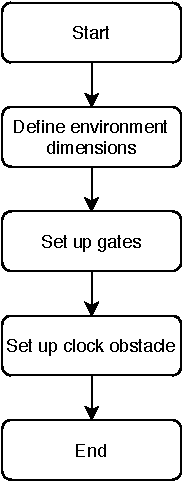
\includegraphics[width=0.3\textwidth]{stationsim_gcs-set_up_station}
    \caption{Flow diagram of process to set up StationSim
    GCS}\label{fig:flow:set_up_station}
\end{figure}

\paragraph{Agent Initialisation}\label{para:submodels:agent_init}

\begin{figure}[h]
    \centering
    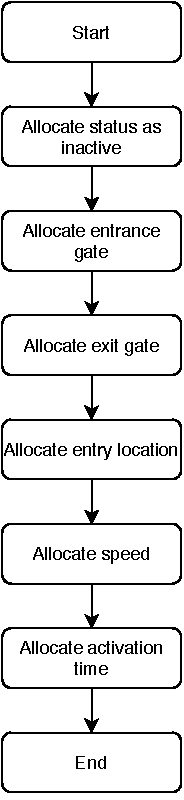
\includegraphics[width=0.3\textwidth]{stationsim_gcs-initialise_agent}
    \caption{Flow diagram of process by which agents are
    initialised}\label{fig:flow:agent_initialisation}
\end{figure}

\paragraph{Agent Entrance Allocation}\label{para:submodels:agent_entrance}

\begin{figure}[h]
    \centering
    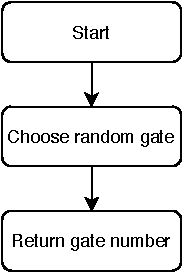
\includegraphics[width=0.2\textwidth]{stationsim_gcs-choose_agent_entrance}
    \caption{Flow diagram of process by which agents' entrance gates are
    selected}\label{fig:flow:agent_entrance}
\end{figure}

\paragraph{Agent Exit Allocation}\label{para:submodels:agent_exit}

\begin{figure}[h]
    \centering
    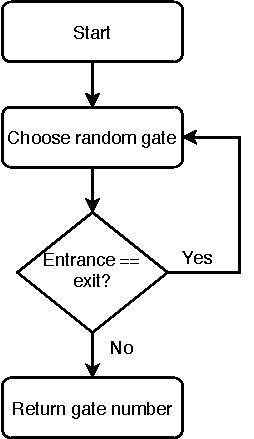
\includegraphics[width=0.3\textwidth]{stationsim_gcs-choose_agent_exit}
    \caption{Flow diagram of process by which agents' exits gates are
    selected}\label{fig:flow:agent_exit}
\end{figure}

\paragraph{Allocating Agent Location based on Gate
Number}\label{para:submodels:location_allocation}

\begin{figure}[h]
    \centering
    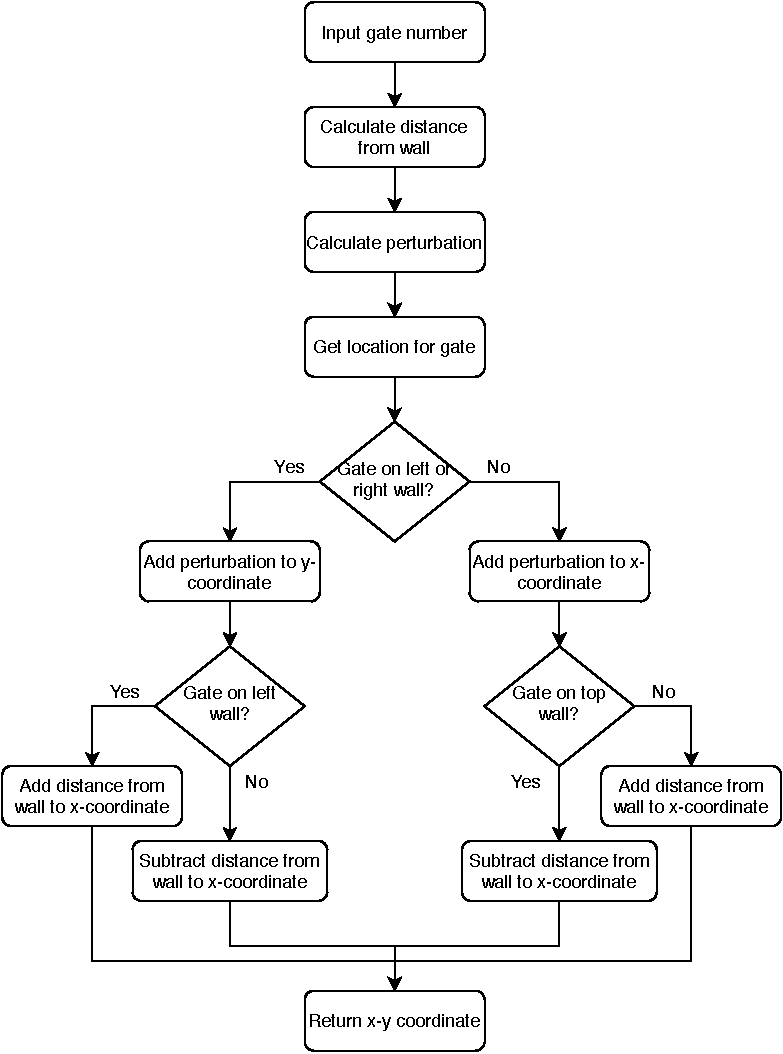
\includegraphics[width=\textwidth]{stationsim_gcs-allocate_agent_location}
    \caption{Flow diagram of process by which an agent's location is allocated
    given a specific gate number; used to allocate initial and final locations
    for agents}\label{fig:flow:allocate_agent_location}
\end{figure}

\paragraph{Allocating Agent Speed}\label{para:submodels:agent_speed}

\begin{figure}[h]
    \centering
    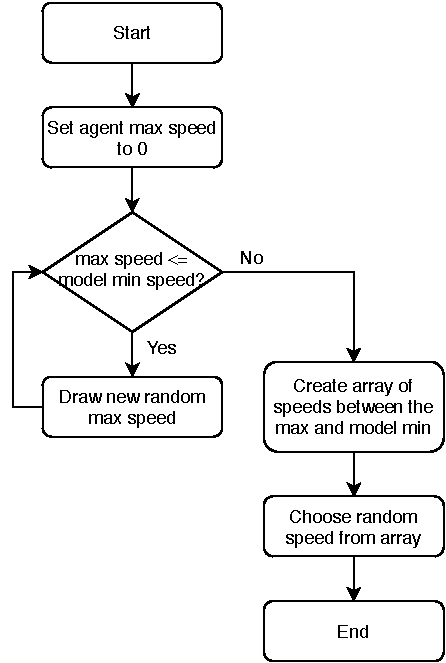
\includegraphics[width=0.5\textwidth]{stationsim_gcs-allocate_agent_speeds}
    \caption{Flow diagram of process by which an agent's speed is
    allocated}\label{fig:flow:allocate_agent_speed}
\end{figure}

\paragraph{Model Step}\label{para:submodels:model_step}

\begin{figure}[h]
    \centering
    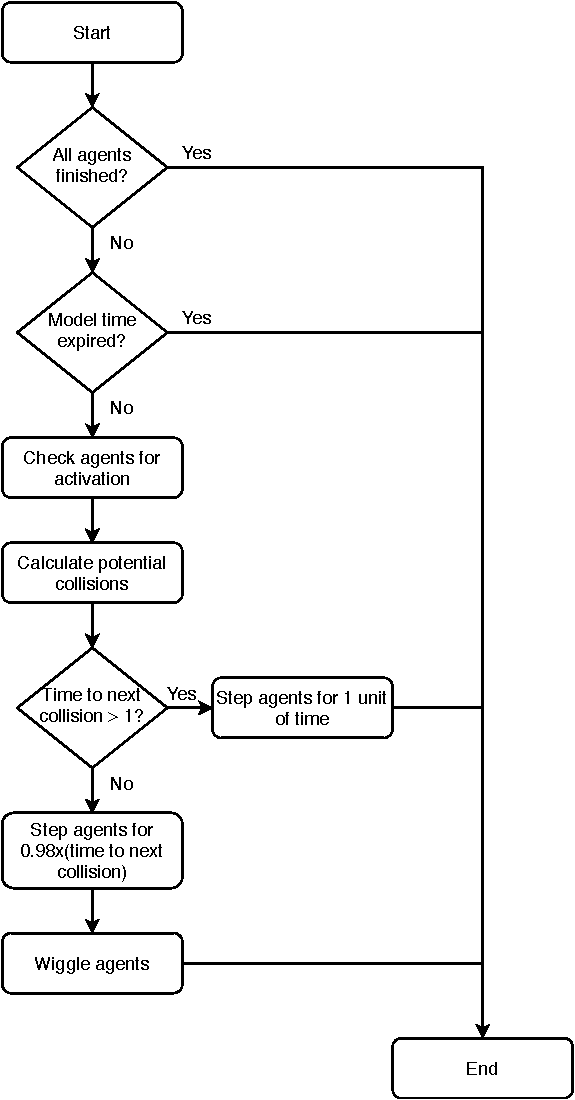
\includegraphics[width=0.8\textwidth]{stationsim_gcs-model_step}
    \caption{Flow diagram of how the model step
    works}\label{fig:flow:model_step}
\end{figure}

\paragraph{Checking for Agent Activation}\label{para:submodels:agent_activation}

\begin{figure}[h]
    \centering
    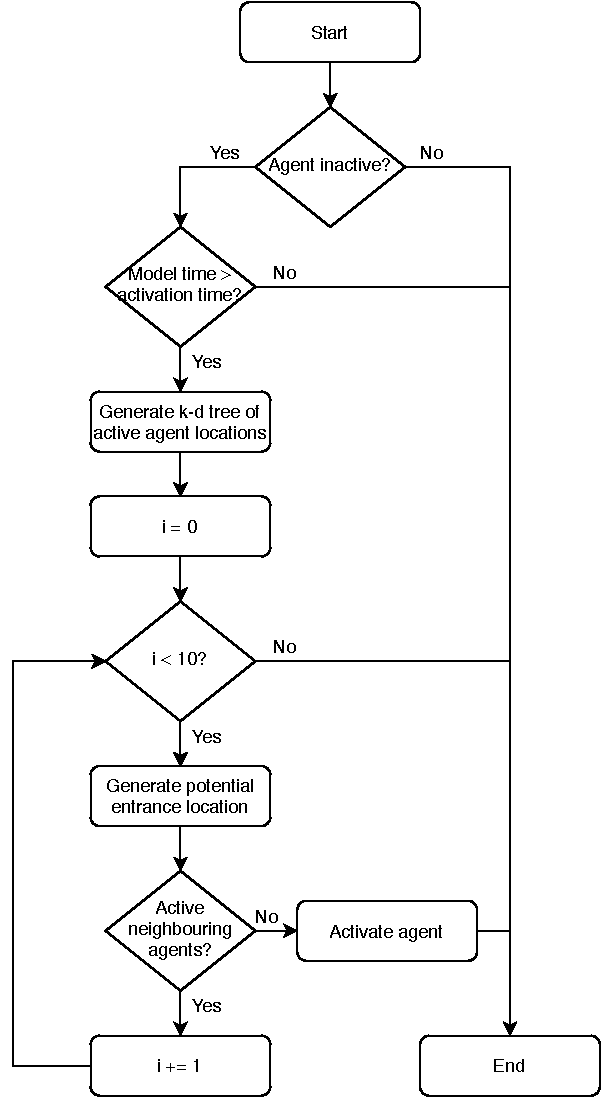
\includegraphics[width=0.8\textwidth]{stationsim_gcs-check_agent_activation}
    \caption{Flow diagram of process to check whether an agent should be
    activated}\label{fig:flow:check_agent_activation}
\end{figure}

\paragraph{Checking for Potential Collisions}\label{para:submodels:collisions}

\begin{figure}[h]
    \centering
    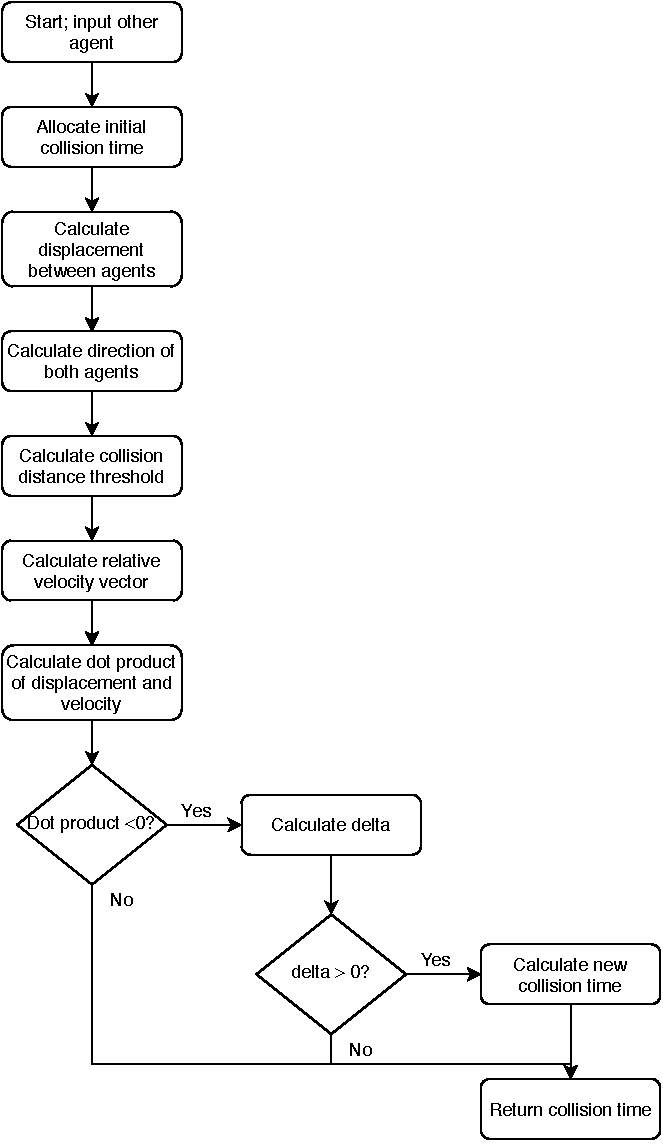
\includegraphics[width=0.8\textwidth]{stationsim_gcs-collisions_agents}
    \caption{Flow diagram of how the time to the next collision between two
    agents is calculated}\label{fig:flow:agent_collisions}
\end{figure}

\begin{figure}[h]
    \centering
    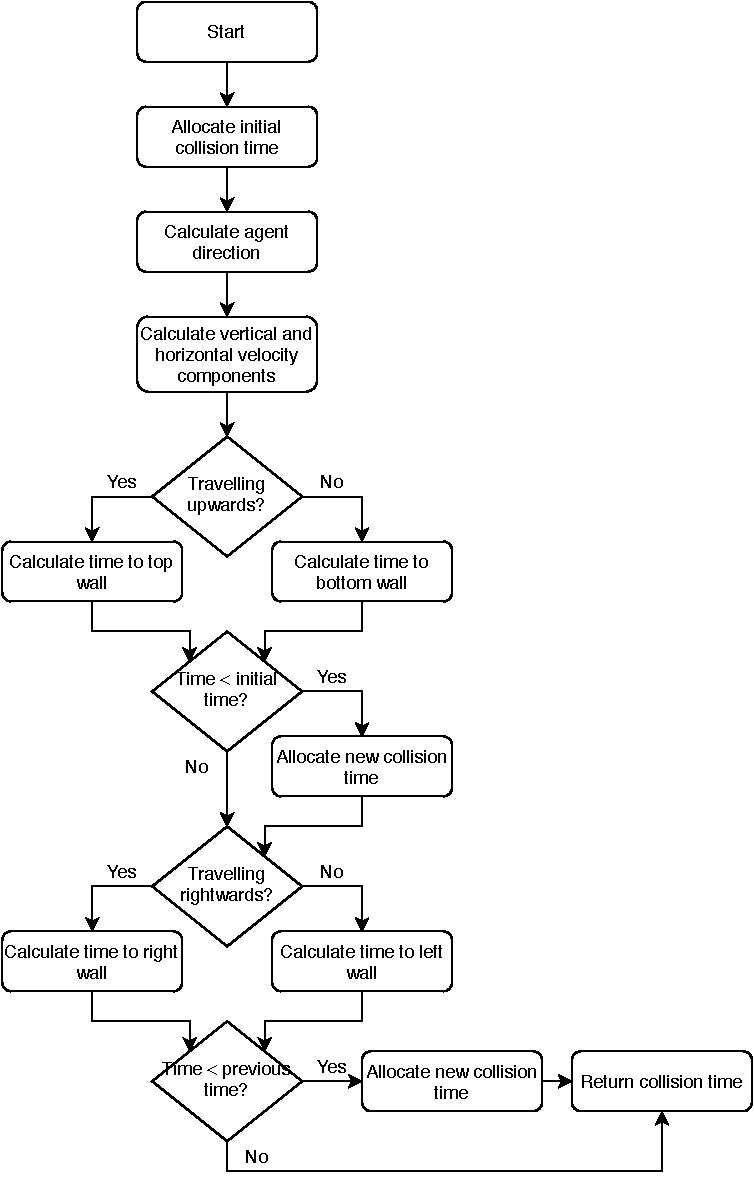
\includegraphics[width=0.9\textwidth]{stationsim_gcs-collisions_walls}
    \caption{Flow diagram of how the time to the next collision between two an
    agent and a wall is calculated}\label{fig:flow:wall_collisions}
\end{figure}

\paragraph{Agent Step}\label{para:submodels:agent_step}

\begin{figure}[h]
    \centering
    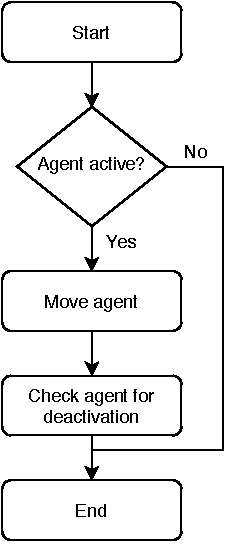
\includegraphics[width=0.4\textwidth]{stationsim_gcs-agent_step}
    \caption{Flow diagram of how the agent step
    works}\label{fig:flow:agent_step}
\end{figure}

\paragraph{Agent Movement}\label{para:submodels:agent_movement}

\begin{figure}[h]
    \centering
    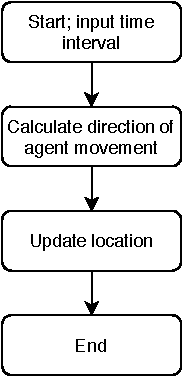
\includegraphics[width=0.4\textwidth]{stationsim_gcs-agent_movement}
    \caption{Flow diagram of how agent movements are
    calculated}\label{fig:flow:agent_movement}
\end{figure}

\paragraph{Agent Wiggle}\label{para:submodels:agent_wiggle}

\begin{figure}[h]
    \centering
    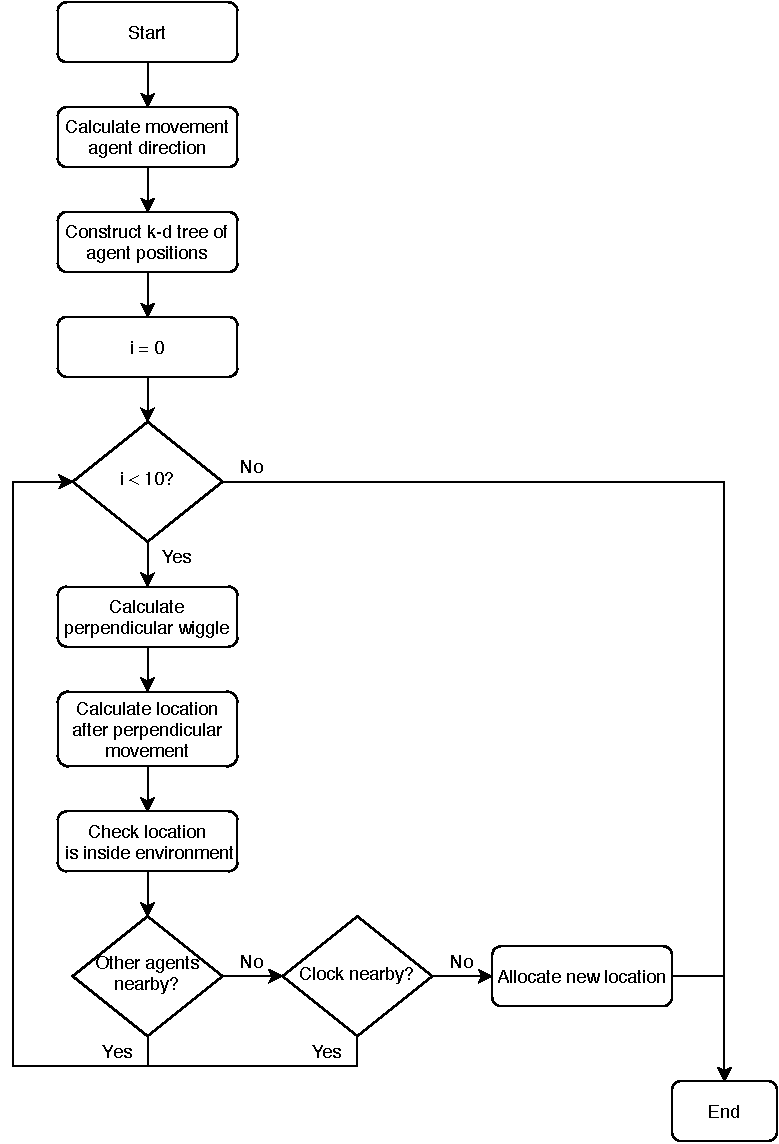
\includegraphics[width=0.8\textwidth]{stationsim_gcs-wiggles}
    \caption{Flow diagram of how agent wiggles are carried
    out}\label{fig:flow:agent_wiggles}
\end{figure}

\paragraph{Checking for Agent
Deactivation}\label{para:submodels:agent_deactivation}

\begin{figure}[h]
    \centering
    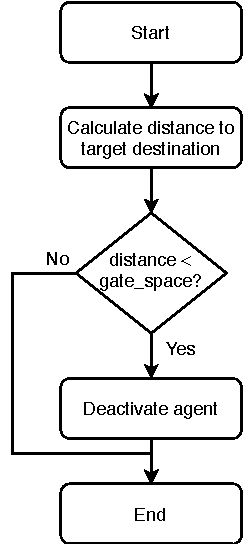
\includegraphics[width=0.4\textwidth]{stationsim_gcs-check_agent_deactivation}
    \caption{Flow diagram of process to check whether an agent should be
    deactivated}\label{fig:flow:check_agent_deactivation}
\end{figure}

\paragraph{Checking for Model
Deactivation}\label{para:submodels:model_deactivation}

